\documentclass[12pt,a4paper]{article}
\usepackage[utf8]{inputenc}
\usepackage{amsmath}
\usepackage{amsfonts}
\usepackage[french]{babel}
\usepackage{amssymb}
\usepackage{graphicx}
\usepackage{palatino}
\usepackage{sectsty}
\usepackage[]{listings}
\usepackage{pgfplots}
\usepackage[french, ruled]{algorithm2e}
%\usepackage{fancyhdr}
\usepackage[colorlinks=true,linkcolor=black]{hyperref}
\usepackage{color}
\usepackage[top=3cm, bottom=3cm, left=2.5cm, right=2.5cm]{geometry}
\pagestyle{plain}
\author{Tafsir GNA}

\lstset{frame=lines, numbers=left,numberstyle=\tiny\bfseries\underline, stepnumber=1, firstnumber =1, numberfirstline=true, backgroundcolor={\color[gray]{0.9}}, showstringspaces=false, basicstyle=\rm\footnotesize}


\makeatletter
\renewcommand{\@algocf@capt@plain}{above}% formerly {bottom}
\makeatother

%\allsectionsfont{\sf}
%\sectionfont{\sffamily\color{black}\sectionrule{3ex}{3pt} %
%{-1.5ex}{1pt}}

\begin{document}

\setcounter{section}{0}

	\begin{titlepage}
		\centering
		
		\noindent%
		
		\begin{minipage}{.15\linewidth}
			
\includegraphics[scale=0.4]{img/ifri_logo.png}
		\end{minipage}
		\hfill
		\begin{minipage}{.68\linewidth}\centering
			\textsc{République du Bénin}\\
			\vspace*{.5cm}
			\textsc{\Large Université d'Abomey-Calavi}
		\end{minipage}
		\hfill
		\begin{minipage}{.15\linewidth}
			
\includegraphics[width=1\linewidth]{img/uac_logo.png}
		\end{minipage}
				
		\vspace{1cm}{\scshape\Large Institut de Formation et de Recherche en Informatique (IFRI)\par}
		\vspace{1cm}{\scshape\Large Mémoire pour l'obtention du diplôme de Master en Systèmes d'Information et Réseaux Informatiques\par}
		\vspace{1.5cm}{\huge\bfseries Résolution de "Pigment Sequencing Problem" avec les algorithmes génétiques\par}
		\vspace{2cm}{\scshape \Large\textbf{Présenté par} \\ Tafsir GNA \par}
		\vfill
		\Large\textbf{Supervisé par}\par Pr. Norbert \textsc{Hounkonnou} \\ \& \\ Dr. Ratheil Vinasétan \textsc{Houndji}
		\vfill
		{\large \scshape Année Académique 2016-2017 \par}
	\end{titlepage}

	\newpage % Page de remerciement
	
	\section*{Remerciements}
	\addcontentsline{toc}{section}{Remerciements}	
	
	\vspace{2.5cm}
	
	Je tiens à remercier tous ceux qui ont aidé et participé à la réalisation de ce travail à travers leurs différents apports et soutiens. \\
	\hspace*{.5cm}Je remercie particulièrement : \\
	\begin{itemize}
		\item[•] Pr. Eugène EZIN, Directeur de l'Institut de Formation et de Recherche en Informatique (IFRI) ainsi que tous les membres du corps enseignant et administratif de l'IFRI;
		\item[•] Pr. Norbert HOUNKONNOU, pour avoir accepté de superviser mes travaux ainsi que Dr. Ratheil HOUNDJI pour l'encadrement et les conseils apportés;
		\item[•] Mon père, ma mère et par extension toute ma famille pour leur soutien et leurs encouragements. 
	\end{itemize}
	
	\newpage
	% Tables des matières
	\tableofcontents
	
	\newpage
	
	%Liste des figures
	\listoffigures
	\addcontentsline{toc}{section}{Liste des figures}
	
	\newpage
	
	%Liste des Tableaux
	\listoftables
	\addcontentsline{toc}{section}{Liste des tableaux}
	
	\newpage
	
	%Liste des algorithmes
	\listofalgorithms
	\addcontentsline{toc}{section}{Liste des algorithmes}
	
	\newpage
	\section*{Glossaire:}
	\addcontentsline{toc}{section}{Glossaire}	
	
	\vspace{1cm}
	
	\label{PSP}\textbf{PSP} : Pigment Sequencing Problem \\
	\hspace*{.5cm} \textbf{AG} : Algorithme Génétique \\
	\hspace*{.5cm} \textbf{F-PGA} : Fine-grained Parallel Genetic Algorithm \\
	\hspace*{.5cm} \textbf{C-PGA} : Coarse-grained Parallel Genetic Algorithm
	
	
	\newpage % Page du résumé en français
	
	\section*{Résumé:}
	\addcontentsline{toc}{section}{Résumé}	
	
	\vspace{1cm}
	
	Le dimensionnement de lot est la tâche la plus difficile et la plus importante dans les problèmes de planification de production en industrie. Il consiste à identifier, sur un horizon de planification, le nombre (et le type) d’articles à produire et à quel moment produire de façon à minimiser le coût total de production. De récentes recherches ont expérimenté une variante NP-Difficile du problème de dimensionnement de lot : le “Pigment Sequencing Problem” (PSP). Aussi, les algorithmes génétiques ont montré leur efficacité sur des problèmes d’optimisation difficiles en trouvant de relatives bonnes solutions par rapport aux solutions optimales. Ce travail vise à donc travers l'application d'une approche heuristique basée sur les algorithmes génétiques au “Pigment Sequencing Problem”, à identifier un plan de production qui respecte les capacités de production des machines tout en minimisant les coûts de stockage et de transition d’une production à une autre. \\
	\\
	\hspace*{.5cm}\textsl{\textbf{Mots clés :}} Algorithme génétique, planification de production, pigment sequencing problem, dimensionnement de lot.
	
	\newpage % Page du résumé en anglais
	
	\section*{Abstract:}
	\addcontentsline{toc}{section}{Abstract}
	
	\vspace{1cm}
	
	The lot sizing is the most difficult and important task in production planning problems in industry field. It involves determining through a planning horizon the number (and the type) of the items to manufacture and when to manufacture these items in order to minimize the overall cost of manufacturing. Some recent researches have experienced a NP-hard variant of lot sizing problem called "Pigment Sequencing Problem" (PSP). Besides, Genetic Algorithms (GA) have shown how effecient they are, in finding some relatively good solutions in comparison to the optimal ones. Thus, This work aims to apply heuristic approach based on genetic algorithms to the Pigment Sequencing Problem, to find a solution that fits into the machine capacity restrictions and that minimizes the stocking costs and change-over costs from one item to another one.\\
	\\
	\hspace*{.5cm}\textsl{\textbf{Key words :}} Genetic algorithm, production planning, pigment sequencing problem, lot sizing.
	
	  
	
	\newpage
	
	\part*{Introduction}
	\addcontentsline{toc}{part}{Introduction}
	
	Dans un processus de planification de production, le dimensionnement
de lots (lot sizing) qui consiste à identifier les articles à produire, quand il
faut les produire et sur quelle machine de façon à satisfaire les demandes
tout en considérant les objectifs financiers, est l’activité la plus importante
et la plus difficile. En effet, de la qualité des décisions qui seront prises
dépendent la performance et la compétitivité de l’entreprise. Connu dans la
littérature sous le nom de problème de lot sizing, il a été beaucoup étudié
ces dernières décennies depuis les travaux de Wagner et Within en 1958. \\
	\hspace*{.5cm} Différentes versions de dimensionnement de lots ont été proposées dans le littérature, chacune étant spécifique à leur domaine d'application. Récemment, (Houndji et al., “The stockingCost constraint”, 2014) et (Ceschia et al., opthub.uniud.it, 2016) ont expérimenté une variante NP-Difficile du problème de dimensionnement de lots. Cette version est connue comme le “Pigment Sequencing Problem” (Pochet et Wolsey 2006, §14.4) et a été récemment inclue à la bibliothèque CSPlib (Gent and Walsh, 1999, prob058) . Il s'agit de produire plusieurs articles avec une seule machine dont la capacité de production est limitée à un article par période. L'horizon de planification est discret et fini, et il y a des coûts de stockage et des coûts de transition d'une production à une autre. Par ailleurs, les demandes sont normalisées et donc binaires. \\
	\hspace*{.5cm} Dans la plupart des cas, un problème d’optimisation tel que le problème de dimensionnement de lots se divise naturellement en deux phases : recherche des solutions admissibles puis recherche de la solution à coût optimal parmi ces dernières. Suivant la méthode employée, ce découpage est plus ou moins apparent dans la résolution. L’usage d’un algorithme génétique est adapté à une exploration rapide et globale d’un espace de recherche de taille importante et est capable de fournir plusieurs solutions. Des calculs effectués ont révélé que l'utilisation des algorithmes génétiques pour des problèmes de dimensionnement de lots semble raisonnable dans le cas de grands problèmes où trouver la solution avec d'autres algorithmes reste encore problématique en temps. Ainsi, Il est possible qu'un algorithme génétique convenablement construit et paramétré puisse trouver de bien meilleurs résultats comparativement à ceux trouvés par d'autres algorithmes tels que le programmation en nombre entier et cela pour un même laps de temps considéré.
	
	\section*{Notre contribution}
	Le "Pigment Sequencing Problem" est un problème NP-Difficile d'optimisation combinatoire pour lequel les instances de taille moyenne peuvent être efficacement résolues en utilisant une formulation appropriée de programmation en nombre mixte. Cependant, dans notre revue de littérature, aucun modèle basé sur les algorithmes génétiques n'a encore été proposé pour ce problème. Nous proposons donc deux méthodes basées sur les algorithmes génétiques pour le problème. La première est une méthode appelée "coarse-grained parallel genetic algorithm" qui divise la population globale en sous-populations. La seconde, appelée "fine-grained parallel genetic algorithm" qui réduit le champ de crossover à l'environnement immédiat. Les tests que nous avons menés afin de valider nos deux méthodes ont produit des résultats satisfaisants et confirmé le fait que les algorithmes génétiques sont efficaces quant il s'agit de problèmes d'optimisation.  
	\section*{Organisation du travail}

	Le travail effectué est organisé dans ce document en 3 parties. Le première partie présente une revue de littérature des problèmes de planification de production, en particulier celui nous concernant, le "Pigment Sequencing Problem" (PSP). Nous présentons également dans cette partie les algorithmes génétiques, leur origine, leurs étapes ainsi que leurs fondements. Dans le deuxième partie, nous présentons dans un premier temps, le modèle ainsi que la formulation utilisée afin de résoudre le problème. Puis dans un second temps, nous explicitons l'approche heuristique utilisée. Dans le chapitre 4, nous expérimentons  notre solution, présentons les résultats obtenus et comparons ces résultats à l'état de l'art en la matière. Pour finir, nous tirons une conclusion du travail effectué et dressons les perspectives possibles en vue d'améliorer ce qui a été fait.
	
	\newpage
	
	\part{Etat de l'art}
	%\newpage
		\section*{Introduction}
		\addcontentsline{toc}{section}{Introduction}
		L'état de l'art revêt une grande importance dans la conduite d'un travail de recherche. Elle permet de fixer les idées quant au travail qui a été déjà fait dans le domaine. Il s'agira donc principalement dans cette première partie de présenter la revue de littérature des problèmes de planification de production, d'exposer les travaux sur les algorithmes génétiques et de montrer en quoi les algorithmes génétiques sont particulièrement adaptés à ces genres de problèmes.
		
	\section{Les problèmes de planification de production}
	La planification de production est un processus qui consiste à déterminer un plan qui indique quelle quantité d'articles produire durant un intervalle de temps appelé "horizon de planification". Il est un important défi pour les entreprises industrielles car il a un fort impact sur leur performance en terme de qualité du service-client et des coûts d'exploitation.	
	
	\subsection{Problématique}
		
 La planification de production s'avère être une tâche très complexe principalement pour les raisons suivantes:
 \begin{itemize}
 	\item[-] Le plus souvent, une ressource de production n'est pas seulement dédiée à un unique article, mais plutôt utilisée pour produire différents types d'articles. Dans un contexte de processus d'industrie, les ressources de production disponibles ne pas vraiment flexibles et ne peuvent produire qu'un type d'article à la fois. En conséquence, la planification de production se heurte à la compétition entre les articles partageant les mêmes ressources et il faut décider quels articles produire, quand et en quelle quantité, tout en prenant en compte les contraintes liées au système de production. Dans certains cas, ces contraintes peuvent être si rigides que trouver une plan de production valide et faisable peut être difficile.
 	
 	\item[-] Un plan de production doit remplir plusieurs objectifs souvent contradictoires, notamment, garantir un excellent niveau du service-client et minimiser la production et les coûts de stockage. Ainsi, les mesures basiques telles que, ne pas satisfaire la demande excédant les capacités de production et garder une haut niveau de stockage afin d'être capable de répondre à toute demande ne sont pas commercialement acceptables ou encore trop chères. Un bon plan de planification est donc le résultat d'un compromis entre différents objectifs contradictoires.
 	\item[-] Un plan de production n'est jamais fixé pour toujours. Sa validité est restreinte à un horizon de planification prédéfini. De plus, la réalité dévie le plus souvent des prévisions et si la divergence entre les plans et les prévisions est trop grande, le plan doit être revu avant la fin de l'horizon de planification.
 \end{itemize}
 
 La planification de production est donc un problème difficile et récurrent pour les compagnies industrielles. Il y a un fort besoin de systèmes d'aide à la décision. Le développement de tels systèmes a été l'objectif d'une grande partie de la littérature en recherche opérationnelle pour les cinquante dernières années. 
	
\subsection{Critères de classification}

Différents critères interviennent dans la classification des problèmes de dimensionnement de lot, notamment : 
\begin{description}
	\item[\textsl{L'échelle de temps}:] La planification peut être effectuée soit sur des périodes discrètes soit sur un
horizon de temps continu. Dans le premier cas, la longueur des périodes peut
être soit de petite taille (Small time buckets) correspondant à des heures ou
jours, soit de grande taille (Big time buckets) correspondant à des jours ou
semaines, soit de très grande taille (Very big time buckets) correspondant à
des mois ou trimestres.

	\item[\textsl{Le nombre de niveaux}:] Dans le cas où seules les demandes venant de l'extérieur du système sont considérées, on parle de problèmes à un niveau. Un état de l'art sur ce type de problème est proposé par Karimi et al. [71]. Lorsqu'il existe une relation entre
les produits, on considère des problèmes à plusieurs niveaux. Ce dernier type
de problèmes se retrouve fréquemment dans l'industrie.

	\item[\textsl{Le nombre de produits}:] Dans le cas où il n'y a pas de dépendance entre les produits, en particulier, s'il n'y a pas d'utilisation commune de la capacité, nous considérons des problèmes
à un seul produit. Dans le cas inverse, on parle de problèmes à plusieurs produits. Un état de l'art sur les problèmes à un produit est proposé par Brahimi
et al. [16].

	\item[\textsl{Les contraintes de capacité}:] Les contraintes de capacité incluent le nombre d'employés, la capacité des machines, la capacité de stockage, etc. Lorsque les contraintes de capacité sont
introduites dans le modèle, elles rendent le problème plus difficile à résoudre,
puisqu'elles lient les produits entre eux.

	\item[\textsl{Les demandes}:] Il existe plusieurs types de demandes qui peuvent être réparties selon trois
groupes :
	\begin{itemize}
		\item[•] Demandes constantes , les valeurs des demandes ne changent pas sur l'horizon de temps, ou demandes dynamiques , les valeurs varient au cours du temps.
		\item[•] Demandes certaines , les valeurs sont connues à l'avance, ou demandes stochastiques , les valeurs sont basées sur des probabilités.
		\item[•] Demandes indépendantes , lorsqu'un produit n'a pas besoin d'autres produits comme composants, ou demandes dépendantes , lorsqu'il existe une relation
entre les produits.
	\end{itemize}

	\item[\textsl{Les coûts et temps de lancement ou préparation (setup)}:] Une ressource peut exécuter des produits de types différents. Ainsi, il est parfois nécessaire de reconfigurer celle-ci à chaque changement de produits. Les coûts et temps induits par le lancement de la ressource sont souvent importants car
élevés et longs.
	
\end{description}

	La complexité des problèmes de dimensionnement de lots varie fortement sous l'influence des différents facteurs comme le nombre de produits, le nombre de niveaux, les contraintes de capacité, etc. Nous avons choisi dans cette étude de décrire les problèmes de dimensionnement de lots selon la longueur de la période de l'horizon de temps. Nous allons donc nous intéresser aux problèmes à courtes et longues périodes.
\subsection{Classes}
	\subsubsection{Problèmes à courtes périodes}
	Ces problèmes (\emph{Small time bucket problems}) sont caractérisés par des périodes de l'ordre de quelques heures, et la séquence des lots lors de la production est prise en compte. Quatre types de problèmes sont étudiés dans la littérature. Pour une étude détaillée de tous ces problèmes, nous pourrons nous référer à Drexl and Kimms [35]. Ces différents types de problèmes sont donc:
	\begin{description}
		\item[\textsl{Discrete lot-sizing and scheduling problem :}]
		Ce problème noté DLSP, est initialement formulé par Fleischmann [43]. La principale hypothèse de ce problème est qu'au plus un article peut être produit par
période. Si un article est fabriqué sur une période, alors toute la capacité disponible sur cette période sera utilisée. Généralement, les coûts de lancement sont pris en compte seulement lorsqu'un nouveau lot commence et non à chaque période.
		\item[\textsl{Continuous setup lot-sizing problem :}]
		Ce problème noté CSLP est similaire au précédent problème. La différence réside dans le fait que lorsqu'un article est produit sur une période, on utilise la capacité nécessaire pour produire cet article et non la capacité entière comme pour le problème précèdent.
		\item[\textsl{Proportional lot-sizing and scheduling problem : }] 
		Dans ce problème, que l'on notera PSLP, la capacité restante pour une période donnée est réutilisée pour produire un second article. Ce problème a été étudié par Drexl et Haase [34] et Kimms et Drexl [78]. Il existe des extensions pour ce problème, par exemple, le cas à plusieurs niveaux et plusieurs machines. Dans [76], Kimms propose de calculer des bornes inférieures, et il résout ce problème à l'aide d'un algorithme génétique dans [77].
		\item[\textsl{General lot-sizing and scheduling problem : }] 
		Ce problème noté GLSP, est plus général que les problèmes précédents, puisque le nombre d'articles à produire par période n'est pas restrictif. Il est étudié par Fleischmann et Meyr [44]. Il existe des extensions de ce problème, par exemple en intégrant des temps de lancement de production dépendant de la séquence des lots à produire ([93]).
	\end{description}
	
	\subsubsection{Problèmes à longues périodes}
	Les problèmes à longues périodes (\emph{Big time bucket problems}) sont basés sur des
horizons de l'ordre de quelques jours à quelques semaines et sont caractérisés par le fait que plus d'un produit peut être fabriqué par période. Nous proposons dans cette section, une étude restreinte de ces problèmes.
	
	\begin{description}
		\item[Les problèmes à un niveau et un produit]: \\
		Ces problèmes ne correspondent pas vraiment à la réalité mais reçoivent beaucoup d'attention et d'intérêt puisque les méthodes mises en œuvre pour les résoudre sont généralisées dans le cas des problématiques à plusieurs niveaux.
		Les premiers travaux sur cette problématique ont été conduits par Manne [90]
et Wagner et Whitin [129]. Leur méthode de résolution est utilisée dans plusieurs
concepts pour résoudre des problèmes plus complexes. Brahimi et al. [16] ont proposé
un état de l'art sur ces problématiques.		
		\item[Les problèmes à un niveau et plusieurs produits]: \\
		Le problème de dimensionnement de lots avec contraintes de capacité est considéré comme un problème complexe puisque la contrainte de capacité engendre un
lien entre les différents produits. Dans le cas où la capacité est considérée comme
infinie, le problème de dimensionnement de lots à N produits est réductible à N
problèmes à un produit et sans capacité, chacun solvable en temps polynomial.
		\item[Les problèmes à plusieurs niveaux]: \\ 
		Ces problèmes sont caractérisés par le fait que les produits finis sont fabriqués à partir de produits intermédiaires. Ainsi, les demandes dépendantes (i.e. les demandes entre les produits) et les demandes indépendantes (i.e. les demandes arrivant de l'extérieur) sont prises en compte dans ce type de problème.
	\end{description}
	
	\begin{center}
		\begin{figure}[!h]
			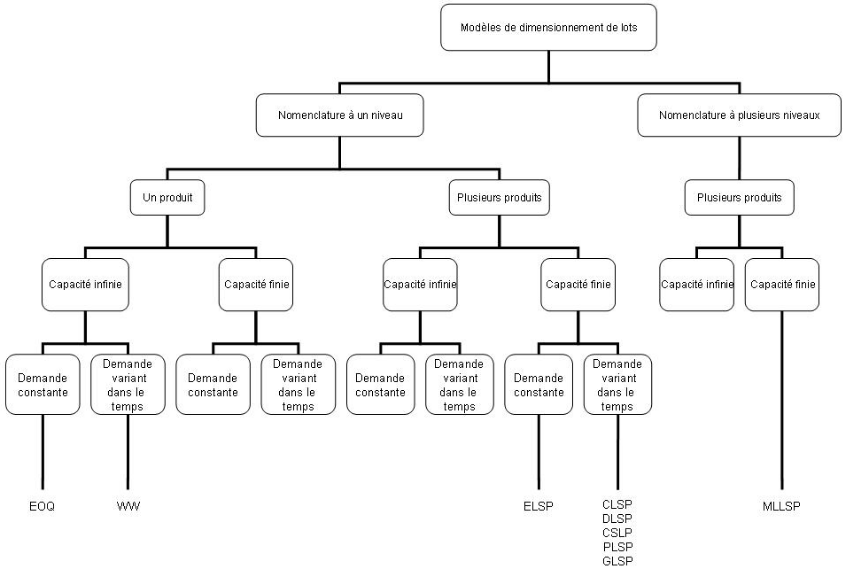
\includegraphics[scale=.5]{img/classification_dimensionnement.png}
			\caption{Exemple de classification des modèles de dimensionnement de lots}
		\end{figure}
	\end{center}

	\newpage
	
	\section{Les algorithmes génétiques}
	Les algorithmes génétiques (AGs) sont des algorithmes d’exploration fondés sur les mécanismes de la sélection naturelle et de la génétique. Ils utilisent à la fois les principes de la survie des structures les mieux adaptées, et les échanges d’informations aléatoires, parfois guidés, pour former un algorithme d’exploration qui possède certaines des caractéristiques de l’exploration humaine. Ils ont été développés par John Holland [7] à l’université du Michigan.
	\subsection{Concepts de base}
	Les AGs constituent une classe de stratégies de recherche réalisant un compromis entre l’exploration et l’exploitation. Ils représentent des méthodes qui utilisent
un choix aléatoire comme outil pour guider une exploration intelligente dans l’espace des paramètres codés. Ce sont des algorithmes itératifs de recherche globale dont l’objectif est d’optimiser une fonction prédéfinie appelée fonction coût ou fonction « fitness » f.
	Les algorithmes génétiques emploient un vocabulaire emprunté à la génétique naturelle. Ils travaillent sur un ensemble d’individus appelé population. Un individu a deux représentations appelées phénotype et génotype. Le phénotype représente une solution potentielle du problème à optimiser en utilisant la formulation originale du problème. Le génotype donne une représentation codée
d’une solution potentielle sous la forme d’un chromosome. Un chromosome est formé de gènes disposés en une succession linéaire et chaque gène peut prendre plusieurs
valeurs appelées allèles. Par exemple, un chromosome se compose d’une succession de 0 et de 1 (c.-à-d. une chaîne binaire), et la valeur pour une certaine position correspond à on (la valeur = 1) ou à off (la valeur = 0) d’un certain dispositif. Des formes plus compliquées, telles qu’un ordre des symboles et une permutation des alphabets, sont choisies pour décrire les chromosomes du problème à optimiser. Chaque individu a une fonction objectif f (fonction « fitness ») qui mesure l’adaptation de l’individu à son environnement local. La théorie darwinienne indique que, parmi des individus d’une population, celui qui est le mieux adapté à l’environnement local a le plus de chance de survivre et d’avoir un plus grand nombre de descendants : c’est la règle de la « survie du plus fort ». Ainsi, la
fonction objectif f du problème d’optimisation joue le rôle d’un critère d’adaptation [18]. Un des points les plus importants des algorithmes génétiques est la flexibilité dans la fonction objectif.

	\subsection{Fonctionnement}
	
	Le principe de fonctionnement de l'algorithme génétique simple est représenté comme suit: \\
	 
	\begin{algorithm}[H]
 	\caption{Algorithme génétique standard}
 	%\KwData{this text}
 	%\KwResult{how to write algorithm with \LaTeX2e }
 	%initialization\;
 	Générer la population initiale Pi \\
 	Évaluer la population Pi \\
 	\While{le critère de terminaison n'est pas satisfait}{
 	 Sélectionner les éléments de Pi à copier dans P i+1 \\
 	 Appliquer le crossover aux éléments de Pi et les mettre dans P i+1 \\
 	 Appliquer la mutation aux éléments de Pi et les mettre dans P i+1 \\
 	 Évaluer la nouvelle population P i+1 \\
 	 Pi = P i+1
 	}
	\end{algorithm}
	
	\vspace*{1cm}
	La figure ci-dessous décrit le processus d'un algorithme génétique simple.
	
	\begin{center}
		\begin{figure}[!h]
			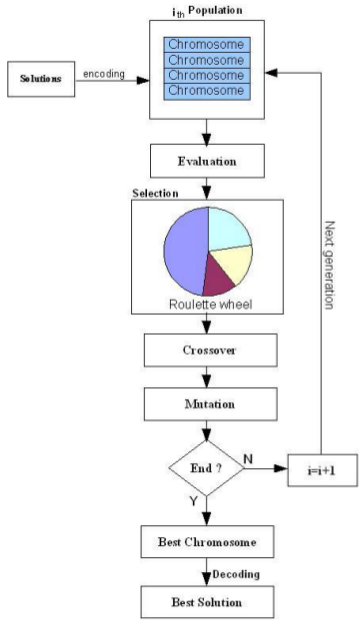
\includegraphics[scale=.6]{img/genetic_algo_flowchart.png}
			\caption{Diagramme d'un algorithme génétique standard}
		\end{figure}
	\end{center}
	
	\newpage
	
	\subsection{Les opérateurs}
		Un algorithme génétique simple utilise les trois opérateurs suivants : la sélection, le croisement et la mutation.
		\subsubsection{L’opérateur de sélection}
		La sélection est un processus dans lequel des individus d’une population sont choisis selon les valeurs de leur fonction coût ou «  fitness  » pour former une nouvelle population. Les individus évoluent par des itérations successives de la sélection, appelées générations. Chaque individu est sélectionné proportionnellement à sa fonction « fitness », donc, un individu avec une fonction « fitness »
plus élevée aura plus de chance d’être sélectionné qu’un autre avec une valeur de « fitness » inférieure. Cette fonction peut être envisagée comme une mesure de profit ou de qualité qu’on souhaite maximiser. Un opérateur simple de sélection est la technique de la roulette pondérée où chaque individu d’une population
occupe une surface de la roulette proportionnelle à la valeur de sa fonction « fitness ». Pour la reproduction, les candidats sont sélectionnés avec une probabilité proportionnelle à leur «  fitness  ». Pour chaque sélection d’un
individu, une simple rotation de la roue donne le candidat sélectionné. Cependant cette sélection n’est pas parfaite. En effet, le risque de favoriser un individu ou un petit ensemble d’individus constitue un inconvénient qui risque d’appauvrir la diversité de la population.
	\subsubsection{L’opérateur de croisement}
	Le croisement est un opérateur de recombinaison. Les individus d’une population sont couplés au hasard par paires représentant les parents. Chaque paire d’individus
subit le croisement décrit comme suit : le croisement opère sur les génotypes (c.-à-d. les chromosomes) de deux individus appelés parents. Il produit de nouveaux individus (généralement deux) appelés enfants dont les gènes sont hérités de l’un ou/et de l’autre parent. Ceci peut être fait en dédoublant chacun des deux chromosomes dans des fragments et en les recombinant pour former de nouveaux chromosomes.
	\begin{description}
		\item[\textsl{Le croisement à un point :}] Si le génotype est une chaîne binaire de longueur n. Le croisement à un point place un point de croisement au
hasard. Un enfant prend une section avant le point de croisement d’un parent et prend l’autre section après le point de croisement de l’autre parent puis recombine les deux sections pour former une nouvelle chaîne binaire. L’autre enfant se construit inversement. Exemple : considérons P1 et P2 deux chaînes binaires de
longueur n = 7 comme parents :
	\begin{center}
		P1 = 0 0 0 0 | 0 0 1 \\
		P2 = 1 1 1 1 | 1 1 0
	\end{center}
	\hspace*{.5cm} Le symbole | indique un point de croisement, dans cet exemple il est placé après le quatrième bit. \\
	\hspace*{.5cm} Le croisement à un point crée les deux nouveaux individus E1 et E2 comme suit :
	\begin{center}
		E1 = 0 0 0 0 | 1 1 0 \\
		E2 = 1 1 1 1 | 0 0 1
	\end{center}
		
		\item[\textsl{Le croisement à deux points :}]Le croisement à deux points place deux points de croisement au hasard, et prend une section entre les points d’un parent et les autres sections en dehors des points de l’autre parent puis les recombine. Dans l’exemple suivant, les deux points de croisement sont placés respectivement après le premier et quatrième bit :
	
	\begin{center}
		P1 = 0 | 0 0 0 | 0 0 1 \\
		P2 = 1 | 1 1 1 | 1 1 0
	\end{center}
	
	Le croisement à deux points résultant rapporte les deux individus suivants :
	\begin{center}
		E1 = 0 | 1 1 1 | 0 0 1 \\
		E2 = 1 | 0 0 0 | 1 1 0
	\end{center}
	
		\item[\textsl{Le croisement uniforme :}]Ce type de croisement a été proposé par Syswerda [14]. Il consiste à choisir avec la même probabilité un allèle de l’un ou de l’autre parent, pour transmettre sa valeur à la même position, aux enfants. Comme le montre l'exemple suivant:
	\begin{center}
		P1 = 0 0 0 0 0 0 1 \\
		P2 = 1 1 1 1 1 1 0 \\
		M = 1 1 0 1 0 0 1
	\end{center}
	
	\begin{center}
		E1 = 0 0 1 0 1 1 1 \\
		E2 = 1 1 0 1 0 0 0
	\end{center}
	
	M représente le masque de transmission dont le principe est le suivant : si la valeur dans le masque est égale à 1, alors la valeur de l’allèle du parent 1 passe à l’enfant 1 (respectivement du parent 2 passe à l’enfant 2) ; sinon la valeur de l’allèle du parent 1 passe à l’enfant 2 (respectivement du parent 2 passe à l’enfant 1), tout en respectant la même position de l’allèle.
	\end{description}
	
	\subsubsection{L'opérateur de mutation}
	
	La mutation opère sur le génotype d’un seul individu. Elle correspond, dans la nature, à une « erreur » qui se produit quand le chromosome est copié et reproduit. Dans une approche numérique, pour une chaîne binaire, elle consiste par exemple à faire pour un allèle un échange entre le « 0 » et le « 1 ». Si des copies exactes sont toujours garanties, alors le taux de mutation est égal à zéro. Cependant, dans la vie réelle, l’erreur de copie peut se produire dans diverses circonstances comme sous l’influence d’un bruit. La mutation change les valeurs de certains gènes avec une faible probabilité. Elle n’améliore pas, en général, les solutions, mais elle évite une perte irréparable de la diversité.
	\begin{center}
		A = 1 0 0 0 0 (avant mutation) \\
		A' = 1 0 1 0 0 (après mutation)
	\end{center}
	
	\subsection{Application des algorithmes génétiques aux problèmes d'optimisation}
	
	Cette approche a été largement utilisée ces dernières années [9, 12, etc.]. L’utilisation des AGs dans de nombreux domaines a fait ses preuves, notamment dans des problèmes combinatoires tels que les problèmes d’ordonnancement [4, 13, 18, 5] et les problèmes de collecte et de distribution. Les problèmes d’ordonnancement d’un atelier classique de type Job-Shop (JSP) ont notamment été largement étudiés et résolus par les AGs [1, 3, 6, 10, 11, 15, etc.]. D’autres algorithmes hybrides ont été aussi proposés [2, 8, 16]. La difficulté principale dans la résolution de ces types de problèmes résulte dans la façon avec laquelle ils sont représentés sous forme algorithmique. Cette phase, la définition du chromosome, représente le point le plus important dans la recherche génétique. Plusieurs approches de représentation
et différents types d’opérateurs d’AGs ont été proposés, pour résoudre ces problèmes.
	
	\section*{Conclusion}
	\addcontentsline{toc}{section}{Conclusion}
	Le dimensionnement de lots en planification de production est un important défi pour les entreprises industrielles. Il consiste à trouver un plan de production qui satisfait aux contraintes spécifiques relatives au système de production. Plusieurs méthodes peuvent servir à résoudre ce problème. Au nombre de ces problèmes, figurent les algorithmes génétiques. Les AGs, à travers l'exploration et l'exploitation de l'espace de recherche ont permis de résoudre bon nombre de problèmes d'optimisation par le passé. Nous proposerons dans la partie suivante deux approches heuristiques basées sur les algorithmes génétiques afin de résoudre le \ref{PSP} PSP, un problème de dimensionnement de lots.
		
	\newpage
	
	\part{Modèle, Formulation et Implémentation}
	
	\setcounter{section}{0}
	
	%\newpage
		\section*{Introduction}
		\addcontentsline{toc}{section}{Introduction}
		L'étude des problèmes de dimensionnement de lots au cours de décennies de recherche a permis de développer différents modèles et formulations correspondant à différents problèmes spécifiques. L'étude du "Pigment Sequencing Problem" (PSP) n'échappe pas à la règle. Dans ce chapitre, nous présentons le modèle mathématique utilisé afin de représenter le problème. Aussi présentons-nous la formulation qui nous a servi à développer notre solution ainsi que la logique qui nous a guidé tout au long de l'implémentation.
		
		\section{Description du problème}
		
		Le PSP consiste à trouver un plan de production
de plusieurs articles à partir d’une machine avec des côuts de changeover . Les
coûts de changeover sont les coûts encourus lors du passage de la production
de l’article i à celui de l’article j avec $i \neq j$. Le plan de production doit
satisfaire les demandes des clients tout en :
	\begin{itemize}
		\item[•] respectant la capacité de production de la machine;
		\item[•] minimisant les coûts de stockage et de changeover.
	\end{itemize}
	\hspace*{.5cm} On suppose que la période de production est suffisamment courte pour ne produire qu’au plus un article par période et que les demandes sont normalisées : la capacité de production de la machine est limitée à un article par
période et d(i, t) $ \in $ {0, 1} avec i l’article et t la période.\\
	\hspace*{.5cm} Il s’agit d’un problème de planification de production ayant les caractéristiques suivantes : un horizon de planification discret et fini ; des contraintes de capacité ; une demande statique et déterministe ; multi-item et small bucket, des coûts de changeover; un seul niveau; sans shortage.\\

	\textbf{\textsl{Illustration}} : Soit un problème avec les données ci-dessous : \\
	\begin{itemize}
		\item[•] Nombre d’articles : $NI = 2$;
		\item[•] Nombre de périodes : $NT = 5$;
		\item[•] Demande par période. Soit d(i, t) la demande de l’article i à la période t : $d(1, t) = (0, 1, 0, 0, 1)$ et $d(2, t) = (1, 0, 0, 0, 1)$;
		\item[•] Coût de stockage. Soit h(i) le coût de stockage de l’article i : $h(1) = h(2) = 2$;
	\end{itemize}
	Soit \emph{xT} le plan de production qui représente une solution potentielle du problème. Il s’agit d’un tableau de dimension \emph{NT} , contenant à son indice t (avec $t  \in  {1...NT}$) l’article i à produire. Une solution admissible du problème est : $ xT = (2, 1, 2, 0, 1)$ avec un coût de $ q(2, 1) + q(1, 2) + q(2, 1) + 2 * h(2) = 15 $. La solution optimale est : $ xT = (2, 1, 0, 1, 2)$ avec un coût de $q(2, 1) + q(1, 2) + h(1) = 10$.
		
		\section{Modèle et formulation}
		Différents modèles ont été proposés afin de représenter les problèmes de planification de production. Suivant le niveau du problème (single-level ou multi-level), le nombre de ressources à considérer (single-resource ou multi-resource) ou que le problème soit encore \emph{small bucket} ou \emph{big bucket}, les modèles en planification de production se rangent dans différentes catégories.   Dans les modèles \emph{small bucket}, au plus un type d'article  peut être produit sur une ressource durant chaque période de temps. Ainsi, un unique article est affecté à chaque période de planification et la séquence d'affectation article-période qui en résulte, définit le plan de production. Aussi dans les modèles \emph{small bucket}, la production d'un lot peut s'étaler sur plusieurs périodes et les coûts de production ne sont pris en compte que s'il y a un nouveau lot à produire. Pour modéliser cela, de nouvelles variables encore appelées variables de \emph{setup} ou variables de \emph{change-over} dans le cas du PSP sont utilisées. \\
		\hspace*{.5cm} Ainsi, le modèle suivant proposé par Pochet et Wolsey (2006, §14.4) s'avère à la fois intéressant et satisfaisant dans le cadre de notre étude.\\
		\\
		\textbf{\textsl{Modèle utilisé}} :
		\begin{eqnarray}
			min \sum_{i,j,t} q^{i,j}ch_{t}^{i,j} + \sum_{i,t} h^{i} s_{t}^{i} \\
			s_{0}^{i} = 0, \forall i \\
			x_{t}^{i} + s_{t-1}^{i} = d_{t}^{i} + s_{t}^{i}, \forall i,t \\
			x_{t}^{i} \leq y_{t}^{i}, \forall i,t \\
			\sum_{i} y_{t}^{i} = 1 , \forall t \\
			ch_{t}^{i,j} = y_{t-1}^{i} + y_{t}^{j} - 1, \forall i,j,t \\
			x,y,ch \in \{0,1\}, s \in N, i \in \{0..NI\}, t \in \{1..NT\}
		\end{eqnarray}
		
		avec les variables de décisions suivantes: \\
		\begin{itemize}
			\item[-] $x_{t}^{i}$ : variable binaire de production qui vaut 1 si l’article i est produit à la période t et 0 sinon ;
			\item[-] $y_{t}^{i}$ : variable binaire de setup qui vaut 1 si la machine est préparée pour la production de l’article i et 0 sinon ;
			\item[-] $s_{t}^{i}$ : variable entière de stockage qui contient le nombre d’articles i stockés à la période t ; 
			\item[-] $ch_{t}^{i,j}$ : variable binaire de changeover qui vaut 1 si à la période t, on est passé de la production de l’article i à l’article j et 0 sinon.
		\end{itemize}
		\vspace*{.3cm}
		\textbf{\textsl{Formulation du modèle}} :\\
		\\
	\hspace*{.5cm} L'objectif est de minimiser la somme des coûts de stockage et des coûts de changeover et est exprimé par la contrainte (1). La contrainte (2) rappelle qu'il n'y a pas de stock initial. La contrainte (3) exprime la règle de la conservation de flot. La contrainte (4) vise à forcer la variable de setup $y_{t}^{i}$ à prendre la valeur 1 s’il y a production de l’article i à la période t. La contrainte (5) s'assure qu'il y a toujours un article qui est préparé. En accord avec la fonction objectif, $y_{t}^{i}$ va prendre la valeur qui minimise le coût de changeover. En général s’il n’y a pas de production à la période t,
$y_{t}^{i} = y_{t-1}^{i}$ ou $y_{t}^{i} = y_{t+1}^{i}$
mais parfois il peut être intéressant de préparer
la machine pour un article intermédiaire sans le produire. La contrainte (6) assigne les valeurs aux variables de changeover.
En effet, si $y_{t-1}^{i}$ et $y_{t}^{i}$ valent 1 alors $ch_{t}^{i,j}$ est obligé de prendre la valeur 1 et sinon $ch_{t}^{i,j}$ serait égale à 0 grâce à la fonction objectif qui minimise le coût de changeover.
		\section{Description de l'approche heuristique proposée}
			\subsection{Représentation génétique}
			\subsection{Initialisation}
			\subsection{Opérateurs génétiques}
				\subsubsection{Sélection}
				\subsubsection{Croisement}
				\subsubsection{Mutation}
			\subsection{Evaluation}
			\subsection{Terminaison}
		
		\section{Fine-grained Parallel Genetic Algorithm}
		\section{Coarse-grained Parallel Genetic Algorithm}
		\section*{Conclusion}
		\addcontentsline{toc}{section}{Conclusion}
		Cette deuxième partie a été l'occasion dans un premier temps d'expliciter le problème du PSP, de présenter le modèle mathématique utilisé ainsi que sa formulation. Dans un second temps, nous avons présenté et détaillé deux approches heuristiques basées sur les algorithmes génétiques utilisée afin de résoudre le problème. La troisième partie sera l'occasion de tester nos deux approches et d'analyser les résultats afin de les comparer à l'état de l'art en la matière.
		
	\newpage
	
	\part{Expérimentations et Analyse des résultats}
	\setcounter{section}{0}
	%\newpage
		\section*{Introduction}
		\addcontentsline{toc}{section}{Introduction}
		L'expérimentation lors d'une étude est une étape importante du travail de recherche. Il s'agit le plus souvent donc de tester les théories émises et d'analyser les résultats obtenus de tests afin de valider nos approches de solution du problème énoncées. Dans cette partie, nous présentons d'abord l'environnement de test, les instances utilisées. Ensuite, nous expérimentons notre solution et à partir des résultats obtenus, nous comparons nos approches heuristiques basées sur les algorithmes génétiques à celles déjà appliquées à ce problème.
		
		\section{Environnement de test} 
		
		\subsection{Matériel}
		Pour l'implémentation de nos tests, nous avons travaillé sur un ordinateur présentant les caractéristiques suivantes :\\
		\begin{itemize}
			\item[•] Système d'exploitation: Linux Ubuntu 16.04 LTS; \\
			\item[•] Processeur: Intel®  Core \up{\textsc{TM}} i7 CPU L 640 @ 2.13GHz x 4; \\
			\item[•] Mémoire: 3,7 Gio;\\
			\item[•] Type du système d'exploitation: 64 bits.\\
		\end{itemize}
		\subsection{Langage de programmation}
		Le langage de programmation utilisée afin de d'implémenter notre solution est le langage \emph{Python} dans sa version Python 3.5. \emph{Python} est un puissant langage de programmation interprété qui apparaît de plus en plus comme une alternative crédible et intéressante dans le domaine de l'intelligence artificielle, tant il présente des qualités quant à sa robustesse, sa rapidité, sa portabilité, sa facilité de prise en main, sa rigueur et sa caractéristique de langage Open source.  
		
		\subsection{Données de test}
		
		Deux ensembles d'instances ont été utilisés dans notre étude afin de tester nos deux solutions. Il s'agit d'une part de celles disponibles dans la bibliothèque \emph{CSPlib} à https://bitbucket.org/ratheilesse/cp4ppet proposées par Houndji et al. (2014). D'autres part, Ceschia et al dans leur application du recuit simulé au PSP ont mis au point un générateur paramétré. Leur générateur reçoit entre autres comme entrées, le nombre d'articles, le nombre de périodes et produit en sortie une instance aléatoire à l'aide de ces paramètres. Ces instances sont disponibles à http://opthub.uniud.it.
		
		\begin{description}
			\item[CSPlib] 
			\item[Opthub]
		\end{description}
		
		\section*{Conclusion}
		\addcontentsline{toc}{section}{Conclusion}
		
	\newpage
		
	\part*{Conclusion et Perspectives}
	\addcontentsline{toc}{part}{Conclusion et Perspectives}
	
	\newpage
	
	\part*{Bibliographie}
	\addcontentsline{toc}{part}{Bibliographie}
	
	\newpage
	
	\appendix
	\part*{Annexes}
	\addcontentsline{toc}{part}{Annexes}
	\section{Extension au problème de planification de production avec plusieurs machines}
		\subsection{Description du problème}
		On s’intéresse ici à un problème de planification de production avec plu-
sieurs machines de capacités finies et constantes. Il y a plusieurs articles à
produire sur un horizon de planification discret et fini. La demande est statique et déterministe et il n’y a pas de shortage. La fonction objectif comprend
les coûts de :
		\begin{itemize}
			\item[•] \emph{setup}: lorsqu’on prépare une machine pour la production d’un article à une période donnée. Ce coût est induit une seule fois
à une période donnée même si on produit plusieurs fois le même article sur la machine ;
			\item[•] \emph{inventory} : lorsqu'on conserve en stocks des articles afin de pouvoir satisfaire les demandes.
		\end{itemize}
		\subsection{Modèle et formulation}
		\subsection{Notre solution}
		\subsection{Expérimentations et Analyse des résultats}
		
	\section{Conception et Structure du programme}
	
	\begin{lstlisting}[language=python]
#!/usr/bin/python3.5
# -*-coding: utf-8 -*

# TODO 
# - give some updates to the implementation of the insertion of the new population into the the former one (test elistism)
# - implement a dynamic values for the parameters depending on the evolution of the algorithm over time
# - another one approach is to take into account the cost of each item to privilegiate a way of implementation of genetic operators 
# - another good clue is to put all the parameters value in a file and pass it as a parameter to the program via this file
# - after a given number of generations without a significative enhancement of the solutions yet found, the thread stops
# - try another way to initialize the population

#--- importation of the modules

from clsp_ga import *
import sys

#---	Start 

# I store the content of the file into an object of Instance class
filename = sys.argv[1]
instance = readFile(filename)

print("-------	Instance of Pigment Sequencing Problem to be used	-------")

print(instance)

# I create an instance of the genetic algorithm to be used
genAlgo = GeneticAlgorithm(instance)

print("-------	Performing the genetic algorithm	--------")

# i store the time when the solving began
startTime = time.clock()

genAlgo.start()

# i store the time when the solving ended
endTime = time.clock()

print(" ")
print("-------	Statistics	-------")
print("time : " + str((endTime - startTime)) + " second(s)")

#---	End
	\end{lstlisting}
	
	\begin{tikzpicture}[scale=0.7]
		\begin{axis}[xlabel=axe $x$, ylabel=axe $y$]
		\addplot {x^2+2*x-1};
		\addlegendentry{une fonction}
		\addplot coordinates {
		(0 ,15)
		(1 ,10)
		(2 ,6)
		(3 ,3)
		(4 ,1)
		(5 ,0)
		};
		\addlegendentry{des données}
		\end{axis}
	\end{tikzpicture}
\end{document}